% Options for packages loaded elsewhere
% Options for packages loaded elsewhere
\PassOptionsToPackage{unicode}{hyperref}
\PassOptionsToPackage{hyphens}{url}
\PassOptionsToPackage{dvipsnames,svgnames,x11names}{xcolor}
%
\documentclass[
  11pt,
  letterpaper,
  DIV=11,
  numbers=noendperiod]{scrartcl}
\usepackage{xcolor}
\usepackage[top=2.5cm,bottom=2.5cm,left=2.5cm,right=2.5cm]{geometry}
\usepackage{amsmath,amssymb}
\setcounter{secnumdepth}{5}
\usepackage{iftex}
\ifPDFTeX
  \usepackage[T1]{fontenc}
  \usepackage[utf8]{inputenc}
  \usepackage{textcomp} % provide euro and other symbols
\else % if luatex or xetex
  \usepackage{unicode-math} % this also loads fontspec
  \defaultfontfeatures{Scale=MatchLowercase}
  \defaultfontfeatures[\rmfamily]{Ligatures=TeX,Scale=1}
\fi
\usepackage{lmodern}
\ifPDFTeX\else
  % xetex/luatex font selection
\fi
% Use upquote if available, for straight quotes in verbatim environments
\IfFileExists{upquote.sty}{\usepackage{upquote}}{}
\IfFileExists{microtype.sty}{% use microtype if available
  \usepackage[]{microtype}
  \UseMicrotypeSet[protrusion]{basicmath} % disable protrusion for tt fonts
}{}
\usepackage{setspace}
\makeatletter
\@ifundefined{KOMAClassName}{% if non-KOMA class
  \IfFileExists{parskip.sty}{%
    \usepackage{parskip}
  }{% else
    \setlength{\parindent}{0pt}
    \setlength{\parskip}{6pt plus 2pt minus 1pt}}
}{% if KOMA class
  \KOMAoptions{parskip=half}}
\makeatother
% Make \paragraph and \subparagraph free-standing
\makeatletter
\ifx\paragraph\undefined\else
  \let\oldparagraph\paragraph
  \renewcommand{\paragraph}{
    \@ifstar
      \xxxParagraphStar
      \xxxParagraphNoStar
  }
  \newcommand{\xxxParagraphStar}[1]{\oldparagraph*{#1}\mbox{}}
  \newcommand{\xxxParagraphNoStar}[1]{\oldparagraph{#1}\mbox{}}
\fi
\ifx\subparagraph\undefined\else
  \let\oldsubparagraph\subparagraph
  \renewcommand{\subparagraph}{
    \@ifstar
      \xxxSubParagraphStar
      \xxxSubParagraphNoStar
  }
  \newcommand{\xxxSubParagraphStar}[1]{\oldsubparagraph*{#1}\mbox{}}
  \newcommand{\xxxSubParagraphNoStar}[1]{\oldsubparagraph{#1}\mbox{}}
\fi
\makeatother


\usepackage{longtable,booktabs,array}
\usepackage{calc} % for calculating minipage widths
% Correct order of tables after \paragraph or \subparagraph
\usepackage{etoolbox}
\makeatletter
\patchcmd\longtable{\par}{\if@noskipsec\mbox{}\fi\par}{}{}
\makeatother
% Allow footnotes in longtable head/foot
\IfFileExists{footnotehyper.sty}{\usepackage{footnotehyper}}{\usepackage{footnote}}
\makesavenoteenv{longtable}
\usepackage{graphicx}
\makeatletter
\newsavebox\pandoc@box
\newcommand*\pandocbounded[1]{% scales image to fit in text height/width
  \sbox\pandoc@box{#1}%
  \Gscale@div\@tempa{\textheight}{\dimexpr\ht\pandoc@box+\dp\pandoc@box\relax}%
  \Gscale@div\@tempb{\linewidth}{\wd\pandoc@box}%
  \ifdim\@tempb\p@<\@tempa\p@\let\@tempa\@tempb\fi% select the smaller of both
  \ifdim\@tempa\p@<\p@\scalebox{\@tempa}{\usebox\pandoc@box}%
  \else\usebox{\pandoc@box}%
  \fi%
}
% Set default figure placement to htbp
\def\fps@figure{htbp}
\makeatother





\setlength{\emergencystretch}{3em} % prevent overfull lines

\providecommand{\tightlist}{%
  \setlength{\itemsep}{0pt}\setlength{\parskip}{0pt}}



 


\usepackage{booktabs}
\usepackage{longtable}
\usepackage{array}
\usepackage{multirow}
\usepackage{wrapfig}
\usepackage{float}
\usepackage{colortbl}
\usepackage{pdflscape}
\usepackage{tabu}
\usepackage{threeparttable}
\usepackage{threeparttablex}
\usepackage[normalem]{ulem}
\usepackage{makecell}
\usepackage{xcolor}
\usepackage{float}
\usepackage{booktabs}
\usepackage{longtable}
\usepackage{array}
\usepackage{multirow}
\usepackage{wrapfig}
\usepackage{colortbl}
\usepackage{pdflscape}
\usepackage{tabu}
\usepackage{threeparttable}
\usepackage{threeparttablex}
\usepackage[normalem]{ulem}
\usepackage{makecell}
\usepackage{xcolor}
\KOMAoption{captions}{tableheading}
\makeatletter
\@ifpackageloaded{caption}{}{\usepackage{caption}}
\AtBeginDocument{%
\ifdefined\contentsname
  \renewcommand*\contentsname{Table of contents}
\else
  \newcommand\contentsname{Table of contents}
\fi
\ifdefined\listfigurename
  \renewcommand*\listfigurename{List of Figures}
\else
  \newcommand\listfigurename{List of Figures}
\fi
\ifdefined\listtablename
  \renewcommand*\listtablename{List of Tables}
\else
  \newcommand\listtablename{List of Tables}
\fi
\ifdefined\figurename
  \renewcommand*\figurename{Figure}
\else
  \newcommand\figurename{Figure}
\fi
\ifdefined\tablename
  \renewcommand*\tablename{Table}
\else
  \newcommand\tablename{Table}
\fi
}
\@ifpackageloaded{float}{}{\usepackage{float}}
\floatstyle{ruled}
\@ifundefined{c@chapter}{\newfloat{codelisting}{h}{lop}}{\newfloat{codelisting}{h}{lop}[chapter]}
\floatname{codelisting}{Listing}
\newcommand*\listoflistings{\listof{codelisting}{List of Listings}}
\makeatother
\makeatletter
\makeatother
\makeatletter
\@ifpackageloaded{caption}{}{\usepackage{caption}}
\@ifpackageloaded{subcaption}{}{\usepackage{subcaption}}
\makeatother
\usepackage{bookmark}
\IfFileExists{xurl.sty}{\usepackage{xurl}}{} % add URL line breaks if available
\urlstyle{same}
\hypersetup{
  pdftitle={Análisis de Perfiles Latentes: Actitudes hacia los Derechos de la Naturaleza},
  colorlinks=true,
  linkcolor={blue},
  filecolor={Maroon},
  citecolor={Blue},
  urlcolor={Blue},
  pdfcreator={LaTeX via pandoc}}


\title{Análisis de Perfiles Latentes: Actitudes hacia los Derechos de la
Naturaleza}
\author{}
\date{2025-08-10}
\begin{document}
\maketitle

\renewcommand*\contentsname{Table of contents}
{
\hypersetup{linkcolor=}
\setcounter{tocdepth}{3}
\tableofcontents
}

\setstretch{1.5}
\newpage

\section{Introducción}\label{introducciuxf3n}

Este documento presenta un análisis de perfiles latentes (Latent Profile
Analysis - LPA) para identificar patrones de respuesta en las actitudes
hacia los derechos de la naturaleza. El conjunto de datos incluye 21
ítems (reducidos de 28 originales) organizados en cuatro ejes
principales:

\begin{itemize}
\tightlist
\item
  \textbf{Base filosófica} (bf): Valores intrínsecos, responsabilidad,
  temporalidad, finalidad
\item
  \textbf{Acción legal} (al): Legitimación, mecanismos, prevención\\
\item
  \textbf{Titular de derechos} (td): Sujeto protegido, jerarquía,
  representación, alcance
\item
  \textbf{Reparación} (rep): Tipo de sanción, enfoque
\end{itemize}

Cada ítem refleja una perspectiva \textbf{antropocéntrica} o
\textbf{biocéntrica}.

\section{Metodología}\label{metodologuxeda}

\subsection{Configuración del
Entorno}\label{configuraciuxf3n-del-entorno}

\subsection{Carga de Datos}\label{carga-de-datos}

\begin{verbatim}
Dimensiones del dataset completo: 143 39 
\end{verbatim}

\begin{verbatim}
Variables disponibles: 39 
\end{verbatim}

\begin{verbatim}
Casos totales: 143 
\end{verbatim}

\subsection{Preparación de los Datos}\label{preparaciuxf3n-de-los-datos}

\begin{verbatim}
Ítems incluidos en el análisis: 21 
\end{verbatim}

\begin{verbatim}
Casos válidos para LPA: 143 
\end{verbatim}

\begin{verbatim}
Ratio casos/variables: 6.81 
\end{verbatim}

\begin{verbatim}
Ítems antropocéntricos: 10 
\end{verbatim}

\begin{verbatim}
Ítems biocéntricos: 11 
\end{verbatim}

\newpage

\section{Resultados}\label{resultados}

\subsection{Características de la
Muestra}\label{caracteruxedsticas-de-la-muestra}

\begin{verbatim}
CARACTERÍSTICAS DE LA MUESTRA
\end{verbatim}

\begin{verbatim}
Edad: Media = 26.3 años (DE = 9.75 )
\end{verbatim}

\begin{verbatim}
Rango de edad: 17 - 66 años
\end{verbatim}

\begin{verbatim}


Table: Características demográficas de la muestra

|Variable        |Categoría |  n| Porcentaje|
|:---------------|:---------|--:|----------:|
|Sexo            |Femenino  |  0|        0.0|
|                |Masculino |  0|        0.0|
|Condición       |Regular   |  0|        0.0|
|                |Irregular |  0|        0.0|
|Nivel Educativo |Pregrado  |  0|        0.0|
|                |Posgrado  | 28|       19.6|
|                |Técnico   |  0|        0.0|
\end{verbatim}

\subsection{Estadísticos Descriptivos de los
Ítems}\label{estaduxedsticos-descriptivos-de-los-uxedtems}

\begin{verbatim}


Table: Estadísticos descriptivos - Parte 1

|           |   n| mean|   sd| min| max|
|:----------|---:|----:|----:|---:|---:|
|q2_bf_ant  | 143| 2.47| 1.07|   1|   5|
|q4_td_bio  | 143| 3.87| 1.11|   1|   5|
|q5_al_bio  | 143| 3.80| 0.90|   1|   5|
|q6_bf_bio  | 143| 3.72| 1.03|   1|   5|
|q7_al_ant  | 143| 2.66| 1.08|   1|   5|
|q8_rep_ant | 143| 2.07| 1.07|   1|   5|
|q9_td_bio  | 143| 3.81| 0.85|   2|   5|
|q10_bf_bio | 143| 3.57| 1.01|   1|   5|
|q11_td_bio | 143| 3.98| 0.83|   1|   5|
|q12_bf_bio | 143| 3.99| 1.01|   1|   5|
\end{verbatim}

\begin{verbatim}


Table: Estadísticos descriptivos - Parte 2

|            |   n| mean|   sd| min| max|
|:-----------|---:|----:|----:|---:|---:|
|q13_al_bio  | 143| 3.76| 0.96|   1|   5|
|q14_rep_bio | 143| 3.95| 0.80|   2|   5|
|q18_rep_ant | 143| 2.33| 0.94|   1|   5|
|q19_td_bio  | 143| 3.94| 1.11|   1|   5|
|q20_bf_ant  | 143| 2.80| 1.27|   1|   5|
|q21_bf_bio  | 143| 3.90| 0.78|   2|   5|
|q22_bf_ant  | 143| 2.67| 1.14|   1|   5|
|q23_td_ant  | 143| 2.59| 1.16|   1|   5|
|q24_td_ant  | 143| 2.62| 1.05|   1|   5|
|q26_td_ant  | 143| 2.49| 1.07|   1|   5|
\end{verbatim}

\subsection{Matriz de Correlaciones}\label{matriz-de-correlaciones}

\begin{figure}[H]

{\centering 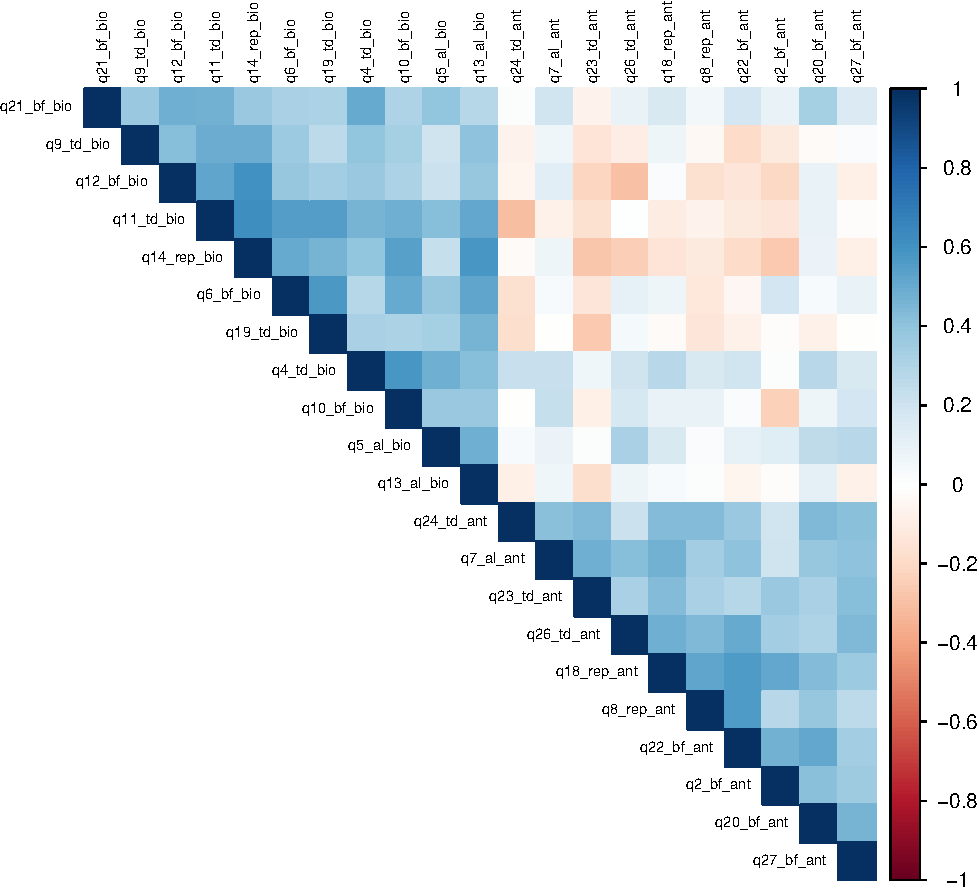
\includegraphics[width=1\linewidth,height=\textheight,keepaspectratio]{analisis_perfiles_latentes_pdf_files/figure-pdf/correlaciones-1.pdf}

}

\caption{Matriz de correlaciones entre ítems}

\end{figure}%

\newpage

\subsection{Análisis de Perfiles
Latentes}\label{anuxe1lisis-de-perfiles-latentes}

\subsubsection{Especificación y Estimación de
Modelos}\label{especificaciuxf3n-y-estimaciuxf3n-de-modelos}

\begin{verbatim}
Casos eliminados por respuestas invariantes: 4 
\end{verbatim}

\begin{verbatim}
Casos válidos para análisis: 139 
\end{verbatim}

\begin{verbatim}
Modelos LPA estimados exitosamente
\end{verbatim}

\subsubsection{Selección del Modelo
Óptimo}\label{selecciuxf3n-del-modelo-uxf3ptimo}

\begin{verbatim}
DIAGNÓSTICO DE MODELOS LPA:
\end{verbatim}

\begin{verbatim}
===========================
\end{verbatim}

\begin{verbatim}
Número de modelos creados: 4 
\end{verbatim}

\begin{verbatim}
Modelo 1 clases:
  - Clase del objeto: tidyProfile.mclust 
  - ¿Tiene atributos?: TRUE 
  - Tipo de objeto: list 
Modelo 2 clases:
  - Clase del objeto: tidyProfile.mclust 
  - ¿Tiene atributos?: TRUE 
  - Tipo de objeto: list 
Modelo 3 clases:
  - Clase del objeto: tidyProfile.mclust 
  - ¿Tiene atributos?: TRUE 
  - Tipo de objeto: list 
Modelo 4 clases:
  - Clase del objeto: tidyProfile.mclust 
  - ¿Tiene atributos?: TRUE 
  - Tipo de objeto: list 
\end{verbatim}

\begin{verbatim}
⚠ Método compare_solutions falló: compare_solutions no funcionó 
Usando método alternativo...

Modelo 1 - Extrayendo estadísticos...
  get_fit no retornó una lista válida
Modelo 2 - Extrayendo estadísticos...
  get_fit no retornó una lista válida
Modelo 3 - Extrayendo estadísticos...
  get_fit no retornó una lista válida
Modelo 4 - Extrayendo estadísticos...
  get_fit no retornó una lista válida
\end{verbatim}

\begin{verbatim}
CRITERIOS DE SELECCIÓN DE MODELO:
\end{verbatim}

\begin{verbatim}
==================================
\end{verbatim}

\begin{verbatim}
⚠ No se pudieron obtener criterios de selección
Procediendo con análisis de 3 perfiles (selección teórica)
\end{verbatim}

\subsubsection{Modelo Final Seleccionado (3
Perfiles)}\label{modelo-final-seleccionado-3-perfiles}

\begin{verbatim}
MODELO SELECCIONADO: 3 perfiles (decisión teórica)
\end{verbatim}

\begin{verbatim}
AIC: NA 
BIC: NA 
Entropía: NA 
\end{verbatim}

\begin{verbatim}
Dimensiones data_lpa_clean: 139 21 
\end{verbatim}

\begin{verbatim}
Calidad de clasificación: Excelente (Entropía ≥ 0.8)
\end{verbatim}

\newpage

\subsection{Características de los
Perfiles}\label{caracteruxedsticas-de-los-perfiles}

\begin{figure}[H]

{\centering 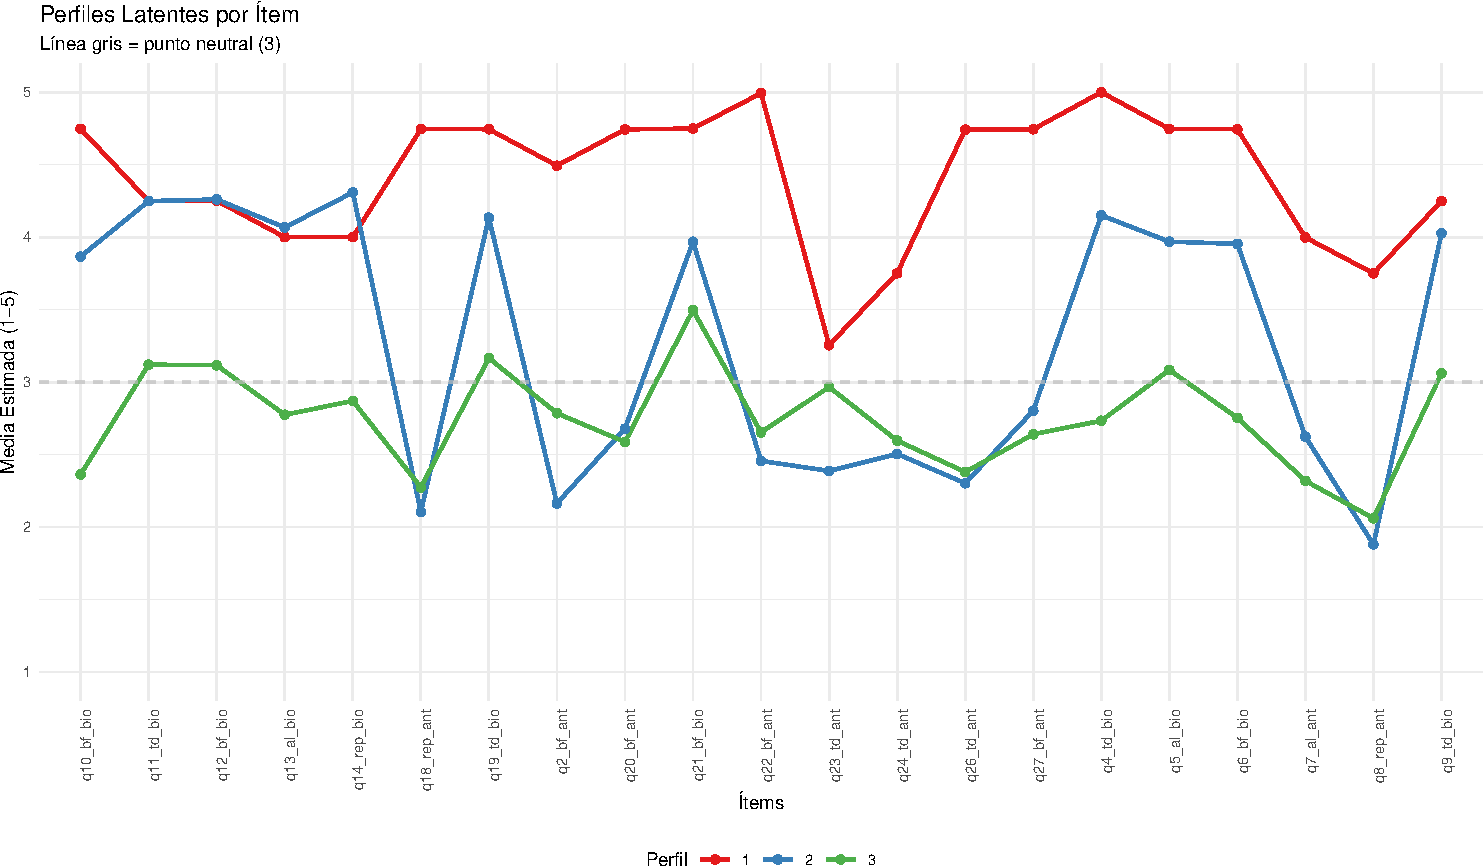
\includegraphics[width=1\linewidth,height=\textheight,keepaspectratio]{analisis_perfiles_latentes_pdf_files/figure-pdf/profile-characteristics-1.pdf}

}

\caption{Perfiles latentes: medias de los ítems por perfil}

\end{figure}%

\begin{verbatim}


Table: Resumen de perfiles por clase

| Class| N_items| Media_General|  Min|  Max|
|-----:|-------:|-------------:|----:|----:|
|     1|      21|          4.41| 3.25| 5.00|
|     2|      21|          3.28| 1.88| 4.31|
|     3|      21|          2.75| 2.06| 3.50|
\end{verbatim}

\subsection{Clasificación de Casos}\label{clasificaciuxf3n-de-casos}

\begin{verbatim}


Table: Distribución de casos por perfil

|Perfil | Frecuencia| Porcentaje|
|:------|----------:|----------:|
|1      |          8|        5.8|
|2      |        100|       71.9|
|3      |         31|       22.3|
\end{verbatim}

\begin{verbatim}


Table: Probabilidades promedio de clasificación

|Perfil | Probabilidad|
|:------|------------:|
|1      |        0.058|
|2      |        0.715|
|3      |        0.227|
\end{verbatim}

\newpage

\section{Interpretación Narrativa}\label{interpretaciuxf3n-narrativa}

\subsection{Caracterización Automática de los
Perfiles}\label{caracterizaciuxf3n-automuxe1tica-de-los-perfiles}

\begin{verbatim}


Table: Caracterización automática de los perfiles

| Perfil|Nombre             |   N| Porcentaje|Orientacion | Media_Ant| Media_Bio|
|------:|:------------------|---:|----------:|:-----------|---------:|---------:|
|      1|Pluralista         |   8|        5.8|Mixta       |      4.32|      4.50|
|      2|Ecocéntrico Fuerte | 100|       71.9|Biocéntrica |      2.39|      4.08|
|      3|Perfil Biocéntrica |  31|       22.3|Biocéntrica |      2.54|      2.95|
\end{verbatim}

\subsection{Análisis por Ejes
Temáticos}\label{anuxe1lisis-por-ejes-temuxe1ticos}

\begin{verbatim}


Table: Medias por eje temático y perfil

|Eje                 | Perfil_1| Perfil_2| Perfil_3|
|:-------------------|--------:|--------:|--------:|
|Acción Legal        |     4.25|     3.55|     2.73|
|Base Filosófica     |     4.69|     3.26|     2.81|
|Reparación          |     4.17|     2.76|     2.40|
|Titular de Derechos |     4.29|     3.39|     2.87|
\end{verbatim}

\subsection{Análisis de Diferencias Entre
Perfiles}\label{anuxe1lisis-de-diferencias-entre-perfiles}

\begin{verbatim}


Table: Los 10 ítems más discriminativos entre perfiles

|Item        | F_statistic| p_value|Significant |
|:-----------|-----------:|-------:|:-----------|
|q14_rep_bio |        92.7|       0|Sí          |
|q10_bf_bio  |        61.5|       0|Sí          |
|q18_rep_ant |        52.9|       0|Sí          |
|q4_td_bio   |        35.3|       0|Sí          |
|q11_td_bio  |        31.0|       0|Sí          |
|q2_bf_ant   |        29.0|       0|Sí          |
|q13_al_bio  |        27.5|       0|Sí          |
|q26_td_ant  |        26.7|       0|Sí          |
|q6_bf_bio   |        25.7|       0|Sí          |
|q22_bf_ant  |        24.9|       0|Sí          |
\end{verbatim}

\begin{verbatim}
ANÁLISIS DETALLADO POR PERFIL
\end{verbatim}

\begin{verbatim}
===============================
\end{verbatim}

\begin{verbatim}
### PERFIL 1 ###
==================

**ÍTEMS DISTINTIVOS ALTOS (>= 4.0):**
-  q4_td_bio  ( Titular de Derechos  -  Biocéntrico ):  5  ( Muy alta )
-  q22_bf_ant  ( Base Filosófica  -  Antropocéntrico ):  4.99  ( Muy alta )
-  q21_bf_bio  ( Base Filosófica  -  Biocéntrico ):  4.75  ( Muy alta )
-  q10_bf_bio  ( Base Filosófica  -  Biocéntrico ):  4.75  ( Muy alta )
-  q5_al_bio  ( Acción Legal  -  Biocéntrico ):  4.75  ( Muy alta )
-  q18_rep_ant  ( Reparación  -  Antropocéntrico ):  4.75  ( Muy alta )
-  q6_bf_bio  ( Base Filosófica  -  Biocéntrico ):  4.74  ( Muy alta )
-  q19_td_bio  ( Titular de Derechos  -  Biocéntrico ):  4.74  ( Muy alta )
-  q27_bf_ant  ( Base Filosófica  -  Antropocéntrico ):  4.74  ( Muy alta )
-  q20_bf_ant  ( Base Filosófica  -  Antropocéntrico ):  4.74  ( Muy alta )
-  q26_td_ant  ( Titular de Derechos  -  Antropocéntrico ):  4.74  ( Muy alta )
-  q2_bf_ant  ( Base Filosófica  -  Antropocéntrico ):  4.49  ( Alta )
-  q12_bf_bio  ( Base Filosófica  -  Biocéntrico ):  4.25  ( Alta )
-  q11_td_bio  ( Titular de Derechos  -  Biocéntrico ):  4.25  ( Alta )
-  q9_td_bio  ( Titular de Derechos  -  Biocéntrico ):  4.25  ( Alta )
-  q13_al_bio  ( Acción Legal  -  Biocéntrico ):  4  ( Alta )
-  q14_rep_bio  ( Reparación  -  Biocéntrico ):  4  ( Alta )

**ÍTEMS MODERADAMENTE ALTOS (3.5-3.99):**
-  q7_al_ant  ( Acción Legal  -  Antropocéntrico ):  4 
-  q24_td_ant  ( Titular de Derechos  -  Antropocéntrico ):  3.75 
-  q8_rep_ant  ( Reparación  -  Antropocéntrico ):  3.75 

**RESUMEN POR ORIENTACIÓN:**
-  Antropocéntrico :  10  ítems, Media =  4.32  (rango:  3.25 - 4.99 )
-  Biocéntrico :  11  ítems, Media =  4.5  (rango:  4 - 5 )

**RESUMEN POR EJE TEMÁTICO:**
-  Base Filosófica : Media =  4.68  ( 8  ítems,  8  altos,  0  bajos)
-  Titular de Derechos : Media =  4.28  ( 7  ítems,  5  altos,  0  bajos)
-  Acción Legal : Media =  4.25  ( 3  ítems,  2  altos,  0  bajos)
-  Reparación : Media =  4.17  ( 3  ítems,  2  altos,  0  bajos)

\newpage

### PERFIL 2 ###
==================

**ÍTEMS DISTINTIVOS ALTOS (>= 4.0):**
-  q14_rep_bio  ( Reparación  -  Biocéntrico ):  4.31  ( Alta )
-  q12_bf_bio  ( Base Filosófica  -  Biocéntrico ):  4.26  ( Alta )
-  q11_td_bio  ( Titular de Derechos  -  Biocéntrico ):  4.25  ( Alta )
-  q4_td_bio  ( Titular de Derechos  -  Biocéntrico ):  4.15  ( Alta )
-  q19_td_bio  ( Titular de Derechos  -  Biocéntrico ):  4.13  ( Alta )
-  q13_al_bio  ( Acción Legal  -  Biocéntrico ):  4.07  ( Alta )
-  q9_td_bio  ( Titular de Derechos  -  Biocéntrico ):  4.03  ( Alta )

**ÍTEMS MODERADAMENTE ALTOS (3.5-3.99):**
-  q5_al_bio  ( Acción Legal  -  Biocéntrico ):  3.97 
-  q21_bf_bio  ( Base Filosófica  -  Biocéntrico ):  3.97 
-  q6_bf_bio  ( Base Filosófica  -  Biocéntrico ):  3.95 
-  q10_bf_bio  ( Base Filosófica  -  Biocéntrico ):  3.87 

**ÍTEMS DISTINTIVOS BAJOS (<= 2.5):**
-  q22_bf_ant  ( Base Filosófica  -  Antropocéntrico ):  2.46  ( Baja )
-  q23_td_ant  ( Titular de Derechos  -  Antropocéntrico ):  2.39  ( Baja )
-  q26_td_ant  ( Titular de Derechos  -  Antropocéntrico ):  2.3  ( Baja )
-  q2_bf_ant  ( Base Filosófica  -  Antropocéntrico ):  2.16  ( Baja )
-  q18_rep_ant  ( Reparación  -  Antropocéntrico ):  2.1  ( Baja )
-  q8_rep_ant  ( Reparación  -  Antropocéntrico ):  1.88  ( Muy baja )

**RESUMEN POR ORIENTACIÓN:**
-  Antropocéntrico :  10  ítems, Media =  2.39  (rango:  1.88 - 2.8 )
-  Biocéntrico :  11  ítems, Media =  4.09  (rango:  3.87 - 4.31 )

**RESUMEN POR EJE TEMÁTICO:**
-  Acción Legal : Media =  3.55  ( 3  ítems,  1  altos,  0  bajos)
-  Titular de Derechos : Media =  3.39  ( 7  ítems,  4  altos,  2  bajos)
-  Base Filosófica : Media =  3.27  ( 8  ítems,  1  altos,  2  bajos)
-  Reparación : Media =  2.76  ( 3  ítems,  1  altos,  2  bajos)

\newpage

### PERFIL 3 ###
==================

**ÍTEMS DISTINTIVOS BAJOS (<= 2.5):**
-  q26_td_ant  ( Titular de Derechos  -  Antropocéntrico ):  2.38  ( Baja )
-  q10_bf_bio  ( Base Filosófica  -  Biocéntrico ):  2.36  ( Baja )
-  q7_al_ant  ( Acción Legal  -  Antropocéntrico ):  2.32  ( Baja )
-  q18_rep_ant  ( Reparación  -  Antropocéntrico ):  2.27  ( Baja )
-  q8_rep_ant  ( Reparación  -  Antropocéntrico ):  2.06  ( Baja )

**RESUMEN POR ORIENTACIÓN:**
-  Antropocéntrico :  10  ítems, Media =  2.53  (rango:  2.06 - 2.97 )
-  Biocéntrico :  11  ítems, Media =  2.96  (rango:  2.36 - 3.5 )

**RESUMEN POR EJE TEMÁTICO:**
-  Titular de Derechos : Media =  2.86  ( 7  ítems,  0  altos,  1  bajos)
-  Base Filosófica : Media =  2.8  ( 8  ítems,  0  altos,  1  bajos)
-  Acción Legal : Media =  2.73  ( 3  ítems,  0  altos,  1  bajos)
-  Reparación : Media =  2.4  ( 3  ítems,  0  altos,  2  bajos)

 - - - - - - - - - - - - - - - - - - - - - - - - - - - - - - - - - - - - - - - - - - - - - - - - - - 
\end{verbatim}

\subsection{Ítems Más Discriminativos - Análisis
Detallado}\label{uxedtems-muxe1s-discriminativos---anuxe1lisis-detallado}

\begin{verbatim}
ÍTEMS MÁS DISCRIMINATIVOS ENTRE PERFILES
\end{verbatim}

\begin{verbatim}
=========================================
\end{verbatim}

\begin{verbatim}
**TOP 12 ÍTEMS MÁS DISCRIMINATIVOS:**
\end{verbatim}

\begin{verbatim}
** 1 .  q14_rep_bio **
   - Eje: Reparación  | Orientación: Biocéntrico 
   - F = 92.7 , p = 0  | Rango = 1.47 
   - Medias: P1 = 4 , P2 = 4.31 , P3 = 2.84 

** 2 .  q10_bf_bio **
   - Eje: Base Filosófica  | Orientación: Biocéntrico 
   - F = 61.5 , p = 0  | Rango = 2.43 
   - Medias: P1 = 4.75 , P2 = 3.87 , P3 = 2.32 

** 3 .  q18_rep_ant **
   - Eje: Reparación  | Orientación: Antropocéntrico 
   - F = 52.9 , p = 0  | Rango = 2.65 
   - Medias: P1 = 4.75 , P2 = 2.1 , P3 = 2.29 

** 4 .  q4_td_bio **
   - Eje: Titular de Derechos  | Orientación: Biocéntrico 
   - F = 35.3 , p = 0  | Rango = 2.29 
   - Medias: P1 = 5 , P2 = 4.15 , P3 = 2.71 

** 5 .  q11_td_bio **
   - Eje: Titular de Derechos  | Orientación: Biocéntrico 
   - F = 31 , p = 0  | Rango = 1.12 
   - Medias: P1 = 4.25 , P2 = 4.24 , P3 = 3.13 

** 6 .  q2_bf_ant **
   - Eje: Base Filosófica  | Orientación: Antropocéntrico 
   - F = 29 , p = 0  | Rango = 2.35 
   - Medias: P1 = 4.5 , P2 = 2.15 , P3 = 2.84 

** 7 .  q13_al_bio **
   - Eje: Acción Legal  | Orientación: Biocéntrico 
   - F = 27.5 , p = 0  | Rango = 1.24 
   - Medias: P1 = 4 , P2 = 4.05 , P3 = 2.81 

** 8 .  q26_td_ant **
   - Eje: Titular de Derechos  | Orientación: Antropocéntrico 
   - F = 26.7 , p = 0  | Rango = 2.45 
   - Medias: P1 = 4.75 , P2 = 2.3 , P3 = 2.39 

** 9 .  q6_bf_bio **
   - Eje: Base Filosófica  | Orientación: Biocéntrico 
   - F = 25.7 , p = 0  | Rango = 1.98 
   - Medias: P1 = 4.75 , P2 = 3.94 , P3 = 2.77 

** 10 .  q22_bf_ant **
   - Eje: Base Filosófica  | Orientación: Antropocéntrico 
   - F = 24.9 , p = 0  | Rango = 2.55 
   - Medias: P1 = 5 , P2 = 2.45 , P3 = 2.68 

** 11 .  q9_td_bio **
   - Eje: Titular de Derechos  | Orientación: Biocéntrico 
   - F = 22.7 , p = 0  | Rango = 1.22 
   - Medias: P1 = 4.25 , P2 = 4.03 , P3 = 3.03 

** 12 .  q5_al_bio **
   - Eje: Acción Legal  | Orientación: Biocéntrico 
   - F = 21.2 , p = 0  | Rango = 1.69 
   - Medias: P1 = 4.75 , P2 = 3.97 , P3 = 3.06 
\end{verbatim}

\begin{verbatim}


Table: Top 8 ítems más discriminativos (compacto)

|Item        | F_stat| Rango| Perfil1| Perfil2| Perfil3|Orientacion     |
|:-----------|------:|-----:|-------:|-------:|-------:|:---------------|
|q14_rep_bio |   92.7|  1.47|    4.00|    4.31|    2.84|Biocéntrico     |
|q10_bf_bio  |   61.5|  2.43|    4.75|    3.87|    2.32|Biocéntrico     |
|q18_rep_ant |   52.9|  2.65|    4.75|    2.10|    2.29|Antropocéntrico |
|q4_td_bio   |   35.3|  2.29|    5.00|    4.15|    2.71|Biocéntrico     |
|q11_td_bio  |   31.0|  1.12|    4.25|    4.24|    3.13|Biocéntrico     |
|q2_bf_ant   |   29.0|  2.35|    4.50|    2.15|    2.84|Antropocéntrico |
|q13_al_bio  |   27.5|  1.24|    4.00|    4.05|    2.81|Biocéntrico     |
|q26_td_ant  |   26.7|  2.45|    4.75|    2.30|    2.39|Antropocéntrico |
\end{verbatim}

\subsection{Patrones Distintivos por
Perfil}\label{patrones-distintivos-por-perfil}

\begin{verbatim}
PATRONES DISTINTIVOS POR PERFIL
\end{verbatim}

\begin{verbatim}
================================
\end{verbatim}

\begin{verbatim}
### PERFIL 1 - PATRONES DISTINTIVOS ###
**Ítems donde este perfil destaca MÁS:**
-  q10_bf_bio  ( Base Filosófica  -  Biocéntrico ):  4.75 
-  q18_rep_ant  ( Reparación  -  Antropocéntrico ):  4.75 
-  q4_td_bio  ( Titular de Derechos  -  Biocéntrico ):  5 
-  q11_td_bio  ( Titular de Derechos  -  Biocéntrico ):  4.25 
-  q2_bf_ant  ( Base Filosófica  -  Antropocéntrico ):  4.5 
-  q26_td_ant  ( Titular de Derechos  -  Antropocéntrico ):  4.75 

 - - - - - - - - - - - - - - - - - - - - - - - - - - - - - - - - - - - - - - - - - - - - - - - - - - 

### PERFIL 2 - PATRONES DISTINTIVOS ###
**Ítems donde este perfil destaca MÁS:**
-  q14_rep_bio  ( Reparación  -  Biocéntrico ):  4.31 
-  q13_al_bio  ( Acción Legal  -  Biocéntrico ):  4.05 
-  q12_bf_bio  ( Base Filosófica  -  Biocéntrico ):  4.26 

**Ítems donde este perfil destaca MENOS:**
-  q18_rep_ant  ( Reparación  -  Antropocéntrico ):  2.1 
-  q2_bf_ant  ( Base Filosófica  -  Antropocéntrico ):  2.15 
-  q26_td_ant  ( Titular de Derechos  -  Antropocéntrico ):  2.3 
-  q22_bf_ant  ( Base Filosófica  -  Antropocéntrico ):  2.45 

 - - - - - - - - - - - - - - - - - - - - - - - - - - - - - - - - - - - - - - - - - - - - - - - - - - 

### PERFIL 3 - PATRONES DISTINTIVOS ###

**Ítems donde este perfil destaca MENOS:**
-  q14_rep_bio  ( Reparación  -  Biocéntrico ):  2.84 
-  q10_bf_bio  ( Base Filosófica  -  Biocéntrico ):  2.32 
-  q4_td_bio  ( Titular de Derechos  -  Biocéntrico ):  2.71 
-  q11_td_bio  ( Titular de Derechos  -  Biocéntrico ):  3.13 

 - - - - - - - - - - - - - - - - - - - - - - - - - - - - - - - - - - - - - - - - - - - - - - - - - - 
\end{verbatim}

\begin{verbatim}
\newpage
\end{verbatim}

\begin{verbatim}
GUÍA PARA INTERPRETACIÓN NARRATIVA
\end{verbatim}

\begin{verbatim}
===================================
\end{verbatim}

\begin{verbatim}
**Criterios para describir cada perfil:**
\end{verbatim}

\begin{verbatim}
1. **Ítems distintivos altos** (>= 4.0): Creencias/actitudes más fuertes
\end{verbatim}

\begin{verbatim}
2. **Ítems distintivos bajos** (<= 2.5): Creencias/actitudes rechazadas
\end{verbatim}

\begin{verbatim}
3. **Patrones por eje temático**: Áreas donde destaca cada perfil
\end{verbatim}

\begin{verbatim}
4. **Orientación predominante**: Tendencia antropocéntrica vs biocéntrica
\end{verbatim}

\begin{verbatim}
5. **Ítems más discriminativos**: Diferencias clave entre perfiles
\end{verbatim}

\begin{verbatim}
**Ejemplo de interpretación:**
\end{verbatim}

\begin{verbatim}
'El Perfil X se caracteriza por [ítems distintivos altos] mientras
\end{verbatim}

\begin{verbatim}
rechaza [ítems distintivos bajos]. Muestra particular fortaleza en
\end{verbatim}

\begin{verbatim}
[eje temático dominante] con orientación [antropo/bio/mixta].'
\end{verbatim}

```

\newpage

\section{Discusión}\label{discusiuxf3n}

\subsection{Hallazgos Principales}\label{hallazgos-principales}

El análisis de perfiles latentes reveló la existencia de \textbf{tres
perfiles distintivos} de actitudes hacia los derechos de la naturaleza
en una muestra de 143 participantes universitarios. Esta tipología
emergente sugiere la presencia de subgrupos con orientaciones
conceptuales diferenciadas respecto a la consideración moral y jurídica
de la naturaleza.

\subsection{Implicaciones
Conceptuales}\label{implicaciones-conceptuales}

\subsubsection{Pluralismo Conceptual}\label{pluralismo-conceptual}

La emergencia de tres perfiles diferenciados evidencia que las actitudes
hacia los derechos de la naturaleza no constituyen un constructo
unidimensional, sino que reflejan \textbf{orientaciones complejas y
multifacéticas}. Esta diversidad conceptual sugiere la necesidad de
aproximaciones pedagógicas y políticas diferenciadas que reconozcan la
pluralidad de marcos interpretativos.

\subsubsection{Tensión
Antropocentrismo-Biocentrismo}\label{tensiuxf3n-antropocentrismo-biocentrismo}

Los perfiles identificados ilustran diferentes formas de
\textbf{negociar la tensión clásica} entre perspectivas antropocéntricas
y biocéntricas en el ámbito jurídico-ambiental. El análisis revela
estrategias diferenciadas para abordar esta dicotomía fundamental.

\subsection{Implicaciones para la Formación
Jurídica}\label{implicaciones-para-la-formaciuxf3n-juruxeddica}

La identificación de perfiles distintivos sugiere la necesidad de
\textbf{estrategias pedagógicas diferenciadas} en la formación jurídica
ambiental. Los estudiantes con diferentes orientaciones conceptuales
pueden beneficiarse de aproximaciones metodológicas específicas que
reconozcan sus marcos interpretativos previos.

\subsection{Limitaciones}\label{limitaciones}

\begin{enumerate}
\def\labelenumi{\arabic{enumi}.}
\tightlist
\item
  \textbf{Generalización}: Muestra de estudiantes universitarios limita
  generalización
\item
  \textbf{Temporalidad}: Estudio transversal no permite inferencias
  causales\\
\item
  \textbf{Contexto cultural}: Resultados específicos al contexto
  socio-cultural
\item
  \textbf{Autoinforme}: Posibles sesgos de deseabilidad social
\end{enumerate}

\subsection{Futuras Líneas de
Investigación}\label{futuras-luxedneas-de-investigaciuxf3n}

\begin{enumerate}
\def\labelenumi{\arabic{enumi}.}
\tightlist
\item
  \textbf{Validación longitudinal} de la estabilidad temporal de los
  perfiles
\item
  \textbf{Estudios comparativos} en diferentes contextos culturales y
  educativos
\item
  \textbf{Factores predictivos} asociados a cada perfil
\item
  \textbf{Intervenciones educativas} basadas en los perfiles
  identificados
\item
  \textbf{Métodos mixtos} para profundizar en la comprensión de cada
  perfil
\end{enumerate}

\section{Conclusiones}\label{conclusiones}

El presente estudio contribuye al entendimiento de la
\textbf{heterogeneidad} en las concepciones estudiantiles sobre los
derechos de la naturaleza. Los hallazgos evidencian la necesidad de
aproximaciones \textbf{multidimensionales} en la investigación y
formación jurídico-ambiental, reconociendo la diversidad de marcos
conceptuales presentes en la población estudiantil.

La identificación de tres perfiles distintivos proporciona una
\textbf{base empírica} para el desarrollo de estrategias educativas
diferenciadas y políticas que consideren la pluralidad de perspectivas
en el ámbito de los derechos de la naturaleza.

\begin{center}\rule{0.5\linewidth}{0.5pt}\end{center}

\textbf{Nota}: Este análisis proporciona una aproximación inicial a los
perfiles latentes de actitudes hacia los derechos de la naturaleza. Los
resultados deben interpretarse considerando el contexto teórico
específico y las limitaciones metodológicas mencionadas.




\end{document}
